\documentclass[a4paper, 11pt]{article}
\usepackage{comment} 
\usepackage{lipsum} %This package just generates Lorem Ipsum filler text. 
\usepackage{fullpage} % changes the margin
\usepackage[a4paper, total={7in, 10in}]{geometry}
\usepackage[fleqn]{amsmath}
\usepackage{amssymb,amsthm}  % assumes amsmath package installed
\newtheorem{theorem}{Theorem}
\newtheorem{corollary}{Corollary}
\usepackage{graphicx}
\usepackage{tikz}
\usetikzlibrary{arrows}
\usepackage{verbatim}
\usepackage[numbered]{mcode}
\usepackage{float}
\usepackage{tikz}
    \usetikzlibrary{shapes,arrows}
    \usetikzlibrary{arrows,calc,positioning}

    \tikzset{
        block/.style = {draw, rectangle,
            minimum height=1cm,
            minimum width=1.5cm},
        input/.style = {coordinate,node distance=1cm},
        output/.style = {coordinate,node distance=4cm},
        arrow/.style={draw, -latex,node distance=2cm},
        pinstyle/.style = {pin edge={latex-, black,node distance=2cm}},
        sum/.style = {draw, circle, node distance=1cm},
    }
\usepackage{xcolor}
\usepackage{mdframed}
\usepackage[shortlabels]{enumitem}
\usepackage{indentfirst}
\usepackage{hyperref}
\usepackage[capitalize, nameinlink]{cleveref}
\renewcommand{\thesubsection}{\thesection.\alph{subsection}}

\newenvironment{problem}[2][Problem]
    { \begin{mdframed}[backgroundcolor=gray!20] \textbf{#1 #2} \\}
    {  \end{mdframed}}

\newenvironment{reduction}
    { \begin{mdframed}[backgroundcolor=blue!20] \\}
    {  \end{mdframed}}
% Define solution environment

\newcommand{\hr}{\noindent\rule{7in}{2.8pt}}
\newenvironment{solution}
    {\textit{Solution:}}
    {\clearpage}
\newcommand{\prob}[1]{\begin{mdframed}[backgroundcolor=gray!20] \textbf{Problem #1}\end{mdframed}}
\renewcommand{\qed}{\quad\qedsymbol}
\newcommand{\bit}{\left\{0, 1\right\}}
\newcommand{\enc}{\mathsf{Enc}}
\newcommand{\dec}{\mathsf{Dec}}
\newcommand{\negl}{\mathsf{negl}}
\newcommand{\prf}{\mathsf{PRFAdv}}
\newcommand{\prg}{\mathsf{PRGAdv}}
\newcommand{\poly}{\mathsf{poly}}
\newcommand{\sign}{\mathsf{Sign}}
\newcommand{\verify}{\mathsf{Verify}}
\newcommand{\macvq}{\mathsf{MAC^{vq}}}
\newcommand{\mac}{\mathsf{MAC}}
\newcommand{\N}{\mathbb{N}}
\newcommand{\R}{\mathbb{R}}
\newcommand{\Z}{\mathbb{Z}}

\newcommand{\calA}{\mathcal{A}}
\newcommand{\calB}{\mathcal{B}}
\newcommand{\calC}{\mathcal{C}}
\newcommand{\calE}{\mathcal{E}}
\newcommand{\calF}{\mathcal{F}}
\newcommand{\calG}{\mathcal{G}}
\newcommand{\calH}{\mathcal{H}}
\newcommand{\calK}{\mathcal{K}}
\newcommand{\calM}{\mathcal{M}}
\newcommand{\calS}{\mathcal{S}}
\newcommand{\calT}{\mathcal{T}}
\newcommand{\calX}{\mathcal{X}}
\newcommand{\calY}{\mathcal{Y}}

\newcommand{\inparen}[1]{\left{ #1 \right}}
\newcommand{\probtwo}[2]{\mathsf{Pr}_{#1}\left[ #2 \right]}
\newcommand{\set}[1]{\left\{ #1 \right\}}
\newcommand{\ct}{\mathsf{ct}}
\newcommand{\twotimessadv}[1]{\mathsf{2SSAdv}\left[ #1 \right]}



\newlength{\protowidth}
\newcommand{\pprotocol}[5]{
{\begin{figure*}[#3]
\begin{center}
\setlength{\protowidth}{\textwidth}
\addtolength{\protowidth}{-3\intextsep}

\fbox{
        \small
        \hbox{\quad
        \begin{minipage}{\protowidth}
    \begin{center}
    {\bf #1}
    \end{center}
        #5
        \end{minipage}
        \quad}

        }
        
\end{center}
\vspace{-4ex}
\caption{{#4} #2}
\end{figure*}
} }

% the first arg is name of security game
% the second arg is caption
% the third arg is the game description
% the label needs to be included 
\newcommand{\securitygame}[4]{
   \pprotocol{#1}{#2}{ht!}{#3}{#4}
}

\newcommand{\constr}[4]{
   \pprotocol{#1}{#2}{tbh!}{#3}{#4}
}

\begin{document}

\noindent
\large\textbf{Anish Banerjee, Shankh Gupta} \hfill \textbf{Problem Set - 2}   \\
\normalsize COL759: Cryptography \hfill September 2023\\
\hr


\prob{1: Cryptosystems secure against side-channel attacks}
\begin{solution}
    Consider the PRF $F':\bit^{n+1}\times\bit^n\rightarrow\bit^n$
    $$F'(k||b_k,x)=
    \begin{cases}
        F(k,0^n)[1\dots n-1]||b_k \hspace{50pt} \text{if } x=0^n  \\
        F(k,x) \hspace{120pt} \text{Otherwise}
    \end{cases}$$
    In other words, the last bit of $F(k,0^n)$ has been replaced with the last bit of the key.

    \begin{enumerate}[(a)]
        \item Let $\calA$ be an adversary which breaks the PRF security of $F'$ with non-negligible advantage $\epsilon$. We will build a reduction $\calB$ which breaks the PRF security of $F$ with the same advantage.
        \securitygame{Problem 1(a)}{Reduction for Problem 1(a)}{\label{red:p1a}}
        {
            \begin{itemize}
                \item Challenger picks a uniformly random bit $b \gets \bit$ and a key $k\gets \calK$.
                \item $\calB$ samples a random $b_k \gets \bit$.
                \item The adversary $\calA$ makes polynomially many queries $\{x_i\}$ to $\calB$ who passes them to the challenger. Challenger replies as in the PRF Game.
                \item Upon receiving the response $y_i$ of each query, $\calB$ checks if $x_i=0$. If so, it modifies $y_i$ by exchanging its last bit with $b_k$. Otherwise, it just passes $y_i$ to $\calA$.
                \item After polynomially many queries, $\calB$ forwards the response send by $\calA$ $(b')$ and wins if $b=b'$.
            \end{itemize}
        }
        \begin{figure}[!ht]
            \centering
            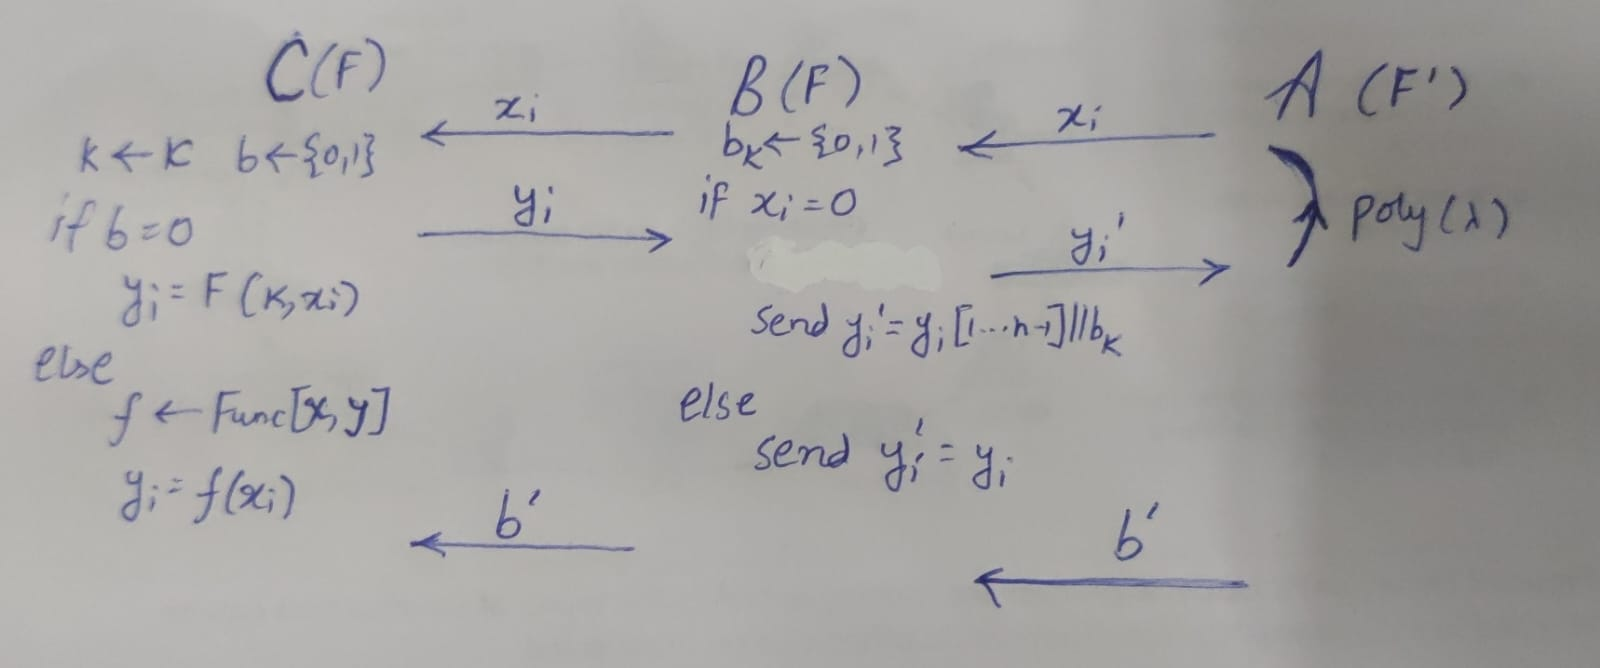
\includegraphics[scale=0.25]{images/Reduction1.jpg}
            \caption{Image for Problem 1(a) Image}
            \label{fig:red1}
        \end{figure}

        When the challenger chooses $b=0$, the game is equivalent to the challenger choosing 0 in PRF game of $F'$. 
        \begin{center}
            Pr[$b'=0|b=0$]=Pr[$\calA$ outputs zero when the challenger chooses 0 in PRF game of $F'$]
        \end{center}
        When the challenger chooses $b=1$, $\calA$ receives the output of a random function for all $x_i\neq0^n$. For $x_i=0^n$, the output received is $r||b_k$. Since $b_k$ is choosen randomly, this too is random.
        \begin{center}
            Pr[$b'=0|b=1$]=Pr[$\calA$ outputs zero when the challenger chooses 1 in PRF game of $F'$]
        \end{center}
        Hence we can conclude,
        $$\prf[\calB,F]=\prf[\calA,F']$$

        \item We will show that $F'$ does not satisfy 1-leakage resilience by constructing an adversary $\calA'$ who makes a leakage query for the last bit of the key and breaks $F'$.
        \begin{itemize}
            \item \textbf{Leakage Query:} $\calA'$ makes a query for the last bit of the key and receives $b_k$ from the challenger.
            \item \textbf{PRF Query:} $\calA'$ queries for the $x=0^n$ and receives $y_i$. He checks if the last bit of $y_i$ is $b_k$. If yes it outputs $b'=0$ (PRF), otherwise it outputs $b'=1$ (Random Function). 
        \end{itemize}
        From the game and definition of $F'$, it is evident that:
        $$\Pr[b'=0|b=0]=1$$
        When the challenger chooses $b=0$, the evaluation of a random function at $0^n$ can have its last bit as 0 or 1 with 1/2 probability. So,
        $$\Pr[b'=0|b=1]=\frac12$$
        And the advantage of $\calA'$ is
        $$\prf[\calA,F']=\Pr[b'=0|b=0]-\Pr[b'=0|b=1]=1-\frac12=\frac12$$
        Which is non-negligible.
    \end{enumerate}
\end{solution}


\prob{2 : MACs: unique queries vs non-unique queries}
\begin{solution}
    
\end{solution}


\prob{3 : A mistake in the lecture notes}
\begin{solution}
    According to the given flawed argument, for any (even unbounded) adversary $\calA$ who wins the MAC game with verification queries ($\macvq$) with advantage $\epsilon$, we can construct an adversary $\calB$ who wins the MAC game without verification queries ($\mac$) with probability $\epsilon$. However, we will show an adversary $\calA'$ who wins  $macvq$ with advantage 1 but the reduction $\calB$ cannot use it to win $\mac$.

    The key observation here is that since every message has a unique signature, $\calB$ cannot send a forgery of a message which it has already queried. 
    \begin{itemize}
        \item $\calA'$ sends verification queries $(\verify , m, \sigma) \forall \sigma\in\calT$ where $\calT$ is the signature space.
        \item For the first verification query, $\calB$ queries the challenger to obtain the signature $\sigma^\star$, and checks all the verification queries against this.
    \end{itemize} 
    One of the queries by $\calA'$ must be $(\verify , m, \sigma^\star)$ and thus he wins the $\macvq$ game. However, $\calB$ cannot use this forgery to win the $\mac$ game since he has already queried it from the challenger.

\end{solution}


\prob{4 : Even-Mansour instantiated with a bad permutation}
\begin{solution}
   
\end{solution}


\prob{5 : 3-round Luby-Rackoff with inversion queries}
\begin{solution}
   
\end{solution}


\prob{6 : CBC mode with bad initialization}
\begin{solution}
   
\end{solution}


\prob{Part B : Theoretical Problem}


\end{document}
